%%%%%%%%%%%%%%%%%%%%%%%%%%%%%%%%%%%%%%%%%
% Undergraduate Thesis for Barrett, The Honors College at Arizona State University
% For the degree of Software Engineering
% By Dylan Lathrum
%
% This document is based on a template by:
% Vel (vel@latextemplates.com)
% Steve Gunn (http://users.ecs.soton.ac.uk/srg/softwaretools/document/templates/)
% Sunil Patel (http://www.sunilpatel.co.uk/thesis-template/)
%
% Under the license:
% CC BY-NC-SA 3.0 (http://creativecommons.org/licenses/by-nc-sa/3.0/)
%
%%%%%%%%%%%%%%%%%%%%%%%%%%%%%%%%%%%%%%%%%

%----------------------------------------------------------------------------------------
%	PACKAGES AND OTHER DOCUMENT CONFIGURATIONS
%----------------------------------------------------------------------------------------

\documentclass[
11pt, % The default document font size, options: 10pt, 11pt, 12pt
% oneside, % Two side (alternating margins) for binding by default, uncomment to switch to one side
english, % ngerman for German
singlespacing, % Single line spacing, alternatives: onehalfspacing or doublespacing
% draft, % Uncomment to enable draft mode (no pictures, no links, overfull hboxes indicated)
final, % Uncomment to enable final mode (hide todos)
%nolistspacing, % If the document is onehalfspacing or doublespacing, uncomment this to set spacing in lists to single
%liststotoc, % Uncomment to add the list of figures/tables/etc to the table of contents
%toctotoc, % Uncomment to add the main table of contents to the table of contents
%parskip, % Uncomment to add space between paragraphs
%nohyperref, % Uncomment to not load the hyperref package
headsepline, % Uncomment to get a line under the header
%chapterinoneline, % Uncomment to place the chapter title next to the number on one line
%consistentlayout, % Uncomment to change the layout of the declaration, abstract and acknowledgements pages to match the default layout
]{MastersDoctoralThesis} % The class file specifying the document structure

\usepackage[utf8]{inputenc} % Required for inputting international characters
\usepackage[T1]{fontenc} % Output font encoding for international characters

\usepackage{mathpazo} % Use the Palatino font by default

\usepackage[backend=bibtex,natbib=true]{biblatex} % Use the bibtex backend

\addbibresource{bibliography.bib} % The filename of the bibliography

\usepackage[autostyle=true]{csquotes} % Required to generate language-dependent quotes in the bibliography

\usepackage{wrapfig} % Required to wrap figures
\usepackage{subcaption} % Required for subfigures

\usepackage[colorinlistoftodos,prependcaption,textsize=tiny,obeyFinal]{todonotes} % Todo notes in margin

\setlength{\marginparwidth}{3cm} % The width of the margin for todo notes
\newcommand{\todoadvisor}[1]{\todo[linecolor=blue,backgroundcolor=blue!25,bordercolor=blue]{#1}}
\newcommand{\todoquestion}[1]{\todo[linecolor=green,backgroundcolor=green!25,bordercolor=green]{#1}}
\newcommand{\todosection}{\todo[linecolor=olive,backgroundcolor=olive!25,bordercolor=olive,inline]{TODO}}

\usepackage{csvsimple} % Import CSV files for use in tables
\usepackage{longtable} % Tables that span multiple pages

\usepackage{listings} % Required for the code examples
% Code block settings
\lstdefinelanguage{custombash}{
	morekeywords={sudo,cp,cd,rm,mv,read,mkdir,cmake,make,makepkg,buildarmimg},
	morestring=[b]{"},
	morestring=[b]{'},
	morecomment=[l]{\#},
	morekeywords=[2]{pkgname,pkgver,pkgrel,\$pkgname,\$pkgver,\$pkgrel},
}
\lstdefinelanguage{customhtml}{
	morekeywords={DOCTYPE,html,lang,head,script,body,let},
	morekeywords=[2]{nextColor,document,body},
	morekeywords=[3]{addEventListener,setAttribute},
	morestring=[b]{"},
	morestring=[b]{'},
	morecomment=[l]{\#},
}
\lstdefinestyle{custombash}{
  language=custombash,
  belowcaptionskip=1\baselineskip,
  breaklines=true,
  frame=single,
	numbers=left,
  % xleftmargin=\parindent,
  showstringspaces=false,
  basicstyle=\footnotesize\ttfamily,
  commentstyle=\itshape\color{green!40!black},
  keywordstyle=\bfseries\color{orange!70!black},
  keywordstyle=[2]\bfseries\color{blue!90!black},
  % identifierstyle=\color{blue},
  stringstyle=\color{orange},
}
\lstdefinestyle{customhtml}{
  language=customhtml,
	morekeywords={uint32_t},
  belowcaptionskip=1\baselineskip,
  breaklines=true,
  frame=single,
  % xleftmargin=\parindent,
	numbers=left,
  showstringspaces=false,
  basicstyle=\footnotesize\ttfamily,
  keywordstyle=\bfseries\color{blue!80!black},
  keywordstyle=[2]\bfseries\color{teal!80!white},
  keywordstyle=[3]\bfseries\color{orange!70!black},
  commentstyle=\itshape\color{green!40!black},
  % identifierstyle=\color{blue},
  stringstyle=\color{orange},
}
\lstdefinestyle{customc}{
  language=C,
	morekeywords={uint32_t},
  belowcaptionskip=1\baselineskip,
  breaklines=true,
  frame=single,
  % xleftmargin=\parindent,
	numbers=left,
  showstringspaces=false,
  basicstyle=\footnotesize\ttfamily,
  keywordstyle=\bfseries\color{blue!80!black},
  commentstyle=\itshape\color{green!40!black},
  % identifierstyle=\color{blue},
  stringstyle=\color{orange},
}
\lstdefinestyle{plaintext}{
  belowcaptionskip=1\baselineskip,
  breaklines=true,
  frame=single,
	numbers=none,
  showstringspaces=false,
  basicstyle=\footnotesize\ttfamily,
}
\lstset{escapechar=@,style=customc}


\usepackage{pgfplots} % Required for the plots
\usepgfplotslibrary{statistics}
\pgfplotsset{compat=1.8}
% Fix mod function bug
% borrowed from <https://tex.stackexchange.com/a/145967/95441>
\pgfmathdeclarefunction{fpumod}{2}{%
		\pgfmathfloatdivide{#1}{#2}%
		\pgfmathfloatint{\pgfmathresult}%
		\pgfmathfloatmultiply{\pgfmathresult}{#2}%
		\pgfmathfloatsubtract{#1}{\pgfmathresult}%
		% replaced `0' by `5' to make it work for this problem
		\pgfmathfloatifapproxequalrel{\pgfmathresult}{#2}{\def\pgfmathresult{5}}{}%
}

\usepackage{chronosys} % Required for timelines

%----------------------------------------------------------------------------------------
%	MARGIN SETTINGS
%----------------------------------------------------------------------------------------

\geometry{
	paper=a4paper, % Change to letterpaper for US letter
	inner=2.5cm, % Inner margin
	outer=3.8cm, % Outer margin
	bindingoffset=.5cm, % Binding offset
	top=1.5cm, % Top margin
	bottom=1.5cm, % Bottom margin
	%showframe, % Uncomment to show how the type block is set on the page
}

%----------------------------------------------------------------------------------------
%	THESIS INFORMATION
%----------------------------------------------------------------------------------------

\thesistitle{Building a Mobile Device that Leverages the Power of a Desktop Computer} % Your thesis title, this is used in the title and abstract, print it elsewhere with \ttitle
\supervisor{Dr. Robert \textsc{Heinrichs}} % Your supervisor's name, this is used in the title page, print it elsewhere with \supname
\examiner{} % Your examiner's name, this is not currently used anywhere in the template, print it elsewhere with \examname
\degree{Software Engineering} % Your degree name, this is used in the title page and abstract, print it elsewhere with \degreename
\author{Dylan \textsc{Lathrum}} % Your name, this is used in the title page and abstract, print it elsewhere with \authorname
\addresses{} % Your address, this is not currently used anywhere in the template, print it elsewhere with \addressname

\subject{Software Engineering} % Your subject area, this is not currently used anywhere in the template, print it elsewhere with \subjectname
\keywords{} % Keywords for your thesis, this is not currently used anywhere in the template, print it elsewhere with \keywordnames
\university{\href{https://www.asu.edu/}{Arizona State University}} % Your university's name and URL, this is used in the title page and abstract, print it elsewhere with \univname
\department{\href{https://barretthonors.asu.edu/}{Barrett, The Honors College}} % Your department's name and URL, this is used in the title page and abstract, print it elsewhere with \deptname
% \group{} % Your research group's name and URL, this is used in the title page, print it elsewhere with \groupname
% \faculty{\href{http://faculty.university.com}{Faculty Name}} % Your faculty's name and URL, this is used in the title page and abstract, print it elsewhere with \facname

\AtBeginDocument{
\hypersetup{pdftitle=\ttitle} % Set the PDF's title to your title
\hypersetup{pdfauthor=\authorname} % Set the PDF's author to your name
\hypersetup{pdfkeywords=\keywordnames} % Set the PDF's keywords to your keywords
}

\begin{document}

\frontmatter % Use roman page numbering style (i, ii, iii, iv...) for the pre-content pages

\pagestyle{plain} % Default to the plain heading style until the thesis style is called for the body content

%----------------------------------------------------------------------------------------
%	TITLE PAGE
%----------------------------------------------------------------------------------------

\begin{titlepage}
	\begin{center}

		\vspace*{.06\textheight}
		{\scshape\LARGE \univname\par}\vspace{1.5cm} % University name
		\textsc{\Large Honors Thesis}\\[0.5cm] % Thesis type

		\HRule \\[0.4cm] % Horizontal line
		{\huge \bfseries \ttitle\par}\vspace{0.4cm} % Thesis title
		\HRule \\[1.5cm] % Horizontal line

		\begin{minipage}[t]{0.4\textwidth}
			\begin{flushleft} \large
				\emph{Author:}\\
				\href{https://www.linkedin.com/in/dylanlathrum/}{\authorname} % Author name - remove the \href bracket to remove the link
			\end{flushleft}
		\end{minipage}
		\begin{minipage}[t]{0.4\textwidth}
			\begin{flushright} \large
				\emph{Director:} \\
				\href{https://isearch.asu.edu/profile/3180015}{\supname} % Supervisor name - remove the \href bracket to remove the link  
			\end{flushright}
		\end{minipage}\\[.5cm]

		\begin{minipage}[t]{0.8\textwidth}
			\begin{flushright} \large
				\emph{Second Reader:}\\
				\href{https://isearch.asu.edu/profile/1232839/}{Ruben Acu\~{n}a}
			\end{flushright}
		\end{minipage}\\[.5cm]
		\begin{minipage}[t]{0.8\textwidth}
			\begin{flushright} \large
				\emph{Third Reader:} \\
				\href{https://isearch.asu.edu/profile/1625795}{Dr. Shawn Jordan}
			\end{flushright}
		\end{minipage}\\[3cm]

		\vfill

		\large \textit{A thesis submitted in fulfillment of the requirements\\ for the degree of \degreename}\\[0.3cm] % University requirement text
		\textit{for}\\[0.4cm]
		\deptname\\[2cm] % Research group name and department name

		\vfill

		{\large \today}\\[4cm] % Date
		%\includegraphics{Logo} % University/department logo - uncomment to place it

		\vfill
	\end{center}
\end{titlepage}

%----------------------------------------------------------------------------------------
%	DECLARATION PAGE
%----------------------------------------------------------------------------------------

\begin{declaration}
	\addchaptertocentry{\authorshipname} % Add the declaration to the table of contents
	\noindent I, \authorname, declare that this thesis titled, \enquote{\ttitle} and the work presented in it are my own. I confirm that:

	\begin{itemize}
		\item This work was done wholly or mainly while in candidature for a research degree at this University.
		\item Where any part of this thesis has previously been submitted for a degree or any other qualification at this University or any other institution, this has been clearly stated.
		\item Where I have consulted the published work of others, this is always clearly attributed.
		\item Where I have quoted from the work of others, the source is always given. With the exception of such quotations, this thesis is entirely my own work.
		\item I have acknowledged all main sources of help.
		\item Where the thesis is based on work done by myself jointly with others, I have made clear exactly what was done by others and what I have contributed myself.\\
	\end{itemize}

	\noindent Signed: Dylan Lathrum\\
	\rule[0.5em]{25em}{0.5pt} % This prints a line for the signature

	\noindent Date: \today\\
	\rule[0.5em]{25em}{0.5pt} % This prints a line to write the date
\end{declaration}

\cleardoublepage

%----------------------------------------------------------------------------------------
%	QUOTATION PAGE
%----------------------------------------------------------------------------------------

\vspace*{0.2\textheight}

\noindent\enquote{\itshape Premature optimization is the root of all evil.}\bigbreak

\hfill Sir Tony Hoare

%----------------------------------------------------------------------------------------
%	ABSTRACT PAGE
%----------------------------------------------------------------------------------------

\begin{abstract}
\addchaptertocentry{\abstractname} % Add the abstract to the table of contents

With the recent focus of attention towards remote work and mobile computing, the possibility of taking a powerful workstation wherever needed is enticing.
However, even emerging laptops today struggle to compete with desktops in terms of cost, maintenance, and future upgrades.
The price point of a powerful laptop is considerably higher compared to an equally powerful desktop computer, and most laptops are manufactured in a way that makes upgrading parts of the machine difficult or impossible, forcing a complete purchase in the event of failure or a component needing an upgrade.

In the case where someone already owns a desktop computer and must be mobile, instead of needing to purchase a second device at full price, it may be possible to develop a low-cost computer that has just enough power to connect to the existing desktop and run all processing there, using the mobile device only as a user interface.

This thesis will explore the development of a custom PCB that utilizes a Raspberry Pi Computer Module 4, as well as the development of a fork of the Open Source project Moonlight to stream a host machine's screen to a remote client.
This implementation will be compared against other existing remote desktop solutions to analyze it's performance and quality.


\end{abstract}

%----------------------------------------------------------------------------------------
%	ACKNOWLEDGEMENTS
%----------------------------------------------------------------------------------------

\begin{acknowledgements}
	\addchaptertocentry{\acknowledgementname} % Add the acknowledgements to the table of contents
	I would like to express my graditude to my thesis director, Dr. Robert Heinrichs, and to each of my committee members, Ruben Acu\~{n}a and Dr. Shawn Jordan, for their help in the development of this thesis.
	Without their guidance, I would not have been able to step so far outside of my comfort zone and learn about so many new topics to make this thesis happen.
	I would also like to thank my friends and family who were always there to bounce ideas off of and inevitably tell me when I was trying to fit too many words into a single section.
\end{acknowledgements}

%----------------------------------------------------------------------------------------
%	LIST OF CONTENTS/FIGURES/TABLES PAGES
%----------------------------------------------------------------------------------------

\tableofcontents % Prints the main table of contents

\listoffigures % Prints the list of figures

\listoftables % Prints the list of tables

%----------------------------------------------------------------------------------------
%	ABBREVIATIONS
%----------------------------------------------------------------------------------------

\begin{abbreviations}{ll} % Include a list of abbreviations (a table of two columns)
	\addchaptertocentry{\abbrevname} % Add the Abbreviations to the table of contents
	\negmedspace % Gets rid of weird extra space
	\textbf{BOM} & \textbf{B}ill \textbf{O}f \textbf{M}aterials\\
	\textbf{CM4} & Raspberry Pi \textbf{C}ompute \textbf{M}odule \textbf{4}\\
	\textbf{CPU} & \textbf{C}entral \textbf{P}rocessing \textbf{U}nit\\
	\textbf{CRD} & \textbf{C}hrome \textbf{R}emote \textbf{D}esktop\\
	\textbf{CSV} & \textbf{C}omma \textbf{S}eparated \textbf{V}alues\\
	\textbf{FFC} & \textbf{F}lat \textbf{F}lexible \textbf{C}able\\
	\textbf{FPS} & \textbf{F}rames \textbf{P}er \textbf{S}econd\\
	\textbf{GPU} & \textbf{G}raphics \textbf{P}rocessing \textbf{U}nit\\
	\textbf{IDE} & \textbf{I}ntegrated \textbf{D}evelopment \textbf{E}nvironment\\
	\textbf{PC} & \textbf{P}ersonal \textbf{C}omputer\\
	\textbf{PCB} & \textbf{P}rinted \textbf{C}ircuit \textbf{B}oard\\
	\textbf{RDP} & \textbf{R}emote \textbf{D}esktop \textbf{P}rotocol\\
	\textbf{RTC} & \textbf{R}eal \textbf{T}ime \textbf{C}lock\\
	\textbf{SBC} & \textbf{S}ingle \textbf{B}oard \textbf{C}omputer\\
	\textbf{SMD} & \textbf{S}urface \textbf{M}ounted \textbf{D}evice\\
	\textbf{SSH} & \textbf{S}ecure \textbf{Sh}ell (Protocol)\\
	\textbf{VNC} & \textbf{V}irtual \textbf{N}etwork \textbf{C}omputing\\

\end{abbreviations}

%----------------------------------------------------------------------------------------
%	PHYSICAL CONSTANTS/OTHER DEFINITIONS
%----------------------------------------------------------------------------------------

% \begin{constants}{lr@{${}={}$}l} % The list of physical constants is a three column table

% 	% The \SI{}{} command is provided by the siunitx package, see its documentation for instructions on how to use it

% 	Speed of Light & $c_{0}$ & \SI{2.99792458e8}{\meter\per\second} (exact)\\
% 	%Constant Name & $Symbol$ & $Constant Value$ with units\\

% \end{constants}

%----------------------------------------------------------------------------------------
%	SYMBOLS
%----------------------------------------------------------------------------------------

% \begin{symbols}{lll} % Include a list of Symbols (a three column table)

% 	$a$ & distance & \si{\meter} \\
% 	$P$ & power & \si{\watt} (\si{\joule\per\second}) \\
% 	%Symbol & Name & Unit \\

% 	\addlinespace % Gap to separate the Roman symbols from the Greek

% 	$\omega$ & angular frequency & \si{\radian} \\

% \end{symbols}

%----------------------------------------------------------------------------------------
%	DEDICATION
%----------------------------------------------------------------------------------------

\dedicatory{For my parents, and their endless support, encouragement, and guidance.}

%----------------------------------------------------------------------------------------
%	THESIS CONTENT - CHAPTERS
%----------------------------------------------------------------------------------------

\mainmatter % Begin numeric (1,2,3...) page numbering

\pagestyle{thesis} % Return the page headers back to the "thesis" style

% Include the chapters of the thesis as separate files from the Chapters folder
% Uncomment the lines as you write the chapters

\chapter{Introduction}

\label{Chapter1}

\section{Power and Portability}

As computers continue to grow to become more and more integrated into our daily lives, purchasing a computer has always been a balance.
Whether its deciding between something cheap or something long-lasting, a machine that is pre-built or a machine that is custom tailored and custom built, or, a tradeoff that has become much more common in recent years, something powerful or something portable.
As with anything, compromises can always be made and a middle ground may be found, but the only way to get the best of both worlds currently is to pay a price premium.
If someone were to look for a computer that is powerful, long-lasting, and upgradable, they would be directed towards a desktop computer.
However, if they needed something with the same power but portable, their only option would be to purchase a laptop costing much more than its desktop counterpart and often with limitations in upgradeability down the line.
Without purchasing both an expensive desktop and an expensive laptop, there currently is no way to get the benefits of both power and portability.


\section{Purpose of this Thesis}

The primary goal of this thesis is to create a portable hardware and software solution that can be used to control a desktop computer remotely while leveraging all of it's power.
There are existing software solutions that give a user remote control of their desktop computer from a different location, but many of them fail to provide a high-quality and performant solution to working with highly demanding programs that put the desktop computer under intense load.
Once attempting to run an intensive application such as rendering video, training Artificial Intelligence, or developing a video game, existing solutions fail to keep up.

In other words, this thesis seeks to provide a user who already owns a powerful desktop computer with a mobile solution that gives them the ability to leverage it's power remotely.


\section{Thesis Overview}

This thesis is split into seven chapters.
Chapter \ref{Chapter2} introduces background knowledge surrounding existing computers, the shift to a more mobile computing world, and the modern day applications for this technology.
Chapter \ref{Chapter3} discusses the current the state of the art in terms of existing solutions for remote computer access, and presents a list of questions that this thesis seeks to answer.
Chapters \ref{Chapter4} and \ref{Chapter5} detail the requirements, design, and production of the hardware and software portions of the project respectively.
This design is tested against the requirements and the existing solutions in Chapter \ref{Chapter6}.
Finally, Chapter \ref{Chapter7} concludes the thesis with a summary of the project's innovations, limitations, and future research.
\chapter{Background} % Main chapter title

\label{Chapter2} % Change X to a consecutive number; for referencing this chapter elsewhere, use \ref{ChapterX}


\section{Specialization of Computers}

\todosection


\subsection{Power of the Desktop}

\todosection


\subsection{Convenience of the Laptop}

\todosection


\subsection{Rise of the Gaming Laptop}

\todosection


\section{Thin Clients}

\todosection


\section{Application to Modern Day}

\todosection
\chapter{State of the Art} % Main chapter title

\label{Chapter3} % Change X to a consecutive number; for referencing this chapter elsewhere, use \ref{ChapterX}

This chapter seeks to provide a summary of existing solutions for remote computer access.
It will not cover specific applications, but rather the protocols that are used to communicate with a remote computer.
Generally speaking, there are two types of solutions that have been developed, software solutions, which are covered in Chapter \ref{sec:SoftwareSolutions} and hardware solutions, which are covered in Chapter \ref{sec:HardwareSolutions}.
Various protocols and implementations are covered in the subsections of those two categories.

\section{Software Solutions}\label{sec:SoftwareSolutions}

While there are many applications in existence that allow a user to remotely control a computer from another location, few of them offer the capabilities required to stream high-performing applications to a remote device.
The following subsections will introduce existing solutions to this problem as well as drawbacks that come with each implementation.


\subsection{Remote Desktop Protocol}\label{subsec:RemoteDesktopProtocol}

Microsoft's Remote Desktop Protocol (RDP), is a protocol that defines communication between a terminal server and terminal server client for multimedia purposes \cite{rdpDocs}.
Coming pre-installed on every Windows machine since Windows XP and with clients available for Windows, Mac, and Linux, RDP is an easy to use solution for remotely accessing Windows machines graphically.

Although it is the built-in solution for Windows machines, it isn't without it's drawbacks.
Firstly, only one graphical session is active at one time while using windows.
This means if a user is logged into the host computer and someone initiates a connection with RDP, the user using the host computer will be logged out.
While this isn't always an issue, sensitive programs that don't take well to being logged out may run into issues.
Secondly, RDP does not support relative mouse movement \cite{burgin_2013}.
This means every mouse input is sent to the host computer as an absolute position on the screen, rather than as a relative distance from it's previous location.
This means any program that moves the user's mouse for them, such as 3D applications with a virtual camera, will be sent the absolute position of the client's mouse.
This will cause the application to detect a large movement of the mouse instantly, which can result in erratic camera movement as the program interprets the mouse moving a large distance every time the cursor is reset to the center of the screen.
Again, while this isn't always an issue, tasks such as 3D modeling and animation or game development cannot be controlled properly.


\subsection{Virtual Network Computing}\label{subsec:VirtualNetworkComputing}

Virtual Network Computing (VNC), is a platform-independent system originally developed by Olivetti \& Oracle Research Labs and later bought and shelved by AT\&T \cite{vncFlavors}.
While the original implementation is no longer used in a wide capacity, the protocol it was developed on has been expanded and improved to become one of the most flexible yet simple ways to control a computer remotely.
VNC can run on any modern operating system, and even a web browser can serve as a VNC client.
It was originally built as the simplest form of remote computer control over LAN, allowing system administrators to control almost any kind of computer with a simple, robust, and extremely compatible system.
However, since its use has gradually outgrown it's original scope, VNC isn't usually the right tool for any job greater than remote system management.
Because of it's simplicity and focus on being as straightforward as possible, VNC is often found to be lacking in terms of security and speed \cite{vncFlavors}.
It is not recommended to use VNC over the internet without some secondary form of security, such as SSL or a secure VPN.


\subsection{Chrome Remote Desktop}\label{subsec:ChromeRemoteDesktop}

Google Chromoting\todo{Should this chapter be called Chromoting? "Chrome Remote Desktop" is the much more recognizable name though}, implemented publicly as Chrome Remote Desktop, is an open source protocol that enables remote desktop control through any web browser running on the Chromium engine \cite{chromotingBuildInstructions}.
It prioritizes low bandwidth usage and ease of access, allowing easy server install on every major desktop operating system, and enables any web browser or mobile device to act as a client.
By employing the VP8 compression format (Most commonly seen in internet video streaming), Chromoting is able to keep network traffic low by only sending a few full images of the server's screen as keyframes and transmitting motion with compressed partial frames \cite{miniorange_chromoting}.
These partial frames are calculated by the server using the difference between the previous and current frame, allowing the server to only send the difference between the two frames.

This save in bandwidth and processing done by the client makes it the perfect solution for Google's ChromeOS laptops coming out around the same time.
These low powered machines were built to be laptops running on the power of a web browser with a link back to more powerful computers when the tasks were too great \cite{upson_sengupta_2012}.
While the protocol works well for remote access, it is limited in certain applications by it's conservative approach to bandwidth usage and reliance on the web browser.


\subsection{Secure Shell Protocol}\label{subsec:SecureShellProtocol}

The Secure Shell Protocol (SSH), is a protocol for securely transmitting data over an insecure network \cite{rfc4251}.
Usually used for remote server management, SSH has become the de facto standard for connecting to a remote computer when nothing more than terminal access is needed.
Paired with the associated SSH file transfer (SFTP) or secure copy (SCP) protocols, SSH provides an incredible amount of flexibility for working with remote computers.
It's largest and most obvious drawback is limited graphical support.
While not a problem for it's traditional use-case, it does limit what high-intensity applications can be used with it.

One recent innovation in remote computing has been the introduction of Remote Development using SSH through the Visual Studio Code IDE.
By opening multiple SSH connections to the host machine at once, Visual Studio Code is able to run the IDE's User interface on the client's machine, and simply send all the written code and commands through to the host machine, utilizing it's power to compile code, run applications, and debug software \cite{vscode_ssh}.
This enables a development experience comparable to working on a local machine by only transmitting the data that is needed over the internet and constructing the visual user interface on the client.
Because of this, high-intensity computational programs such as Artificial Intelligence training and simulation can be run on a powerful host machine and only need to transmit the output to the lower-powered client, but graphical applications are still limited.

\section{Hardware Solutions}\label{sec:HardwareSolutions}

While Hardware solutions are not as popular or widespread as software solutions, there has been some innovation in the field that is worth considering.
Hardware solutions usually focus on building a device that has just enough power to connect and stream data to a remote computer in order to leverage its power for the user to use.


\subsection{Thin Clients}\label{subsec:ThinClients}

As discussed in Section \ref{sec:ThinClients}, Thin Clients are a family of devices commonly seen in the corporate world to allow employees to access data centers and computing clusters from their desks.
Due to their low cost and ease of deployment, they are often the device of choice to enable employees to access the full power of the business' computing infrastructure without needed to purchase a powerful device for each employee.
However, since a typical thin client is a headless device, meaning it doesn't come with a monitor, keyboard, mouse, or other peripherals, they are often less portable as one might think.
A thin client is usually set up once, and then left in that place for as long as a desktop would stay.
Especially with laptop sales on the rise, thin clients do not have the benefit of being more portable than the alternatives.

\subsection{Nvidia Shield and GameStream}\label{subsec:NvidiaShieldAndGameStream}

\begin{wrapfigure}{r}{0.375\textwidth}
  \centering
  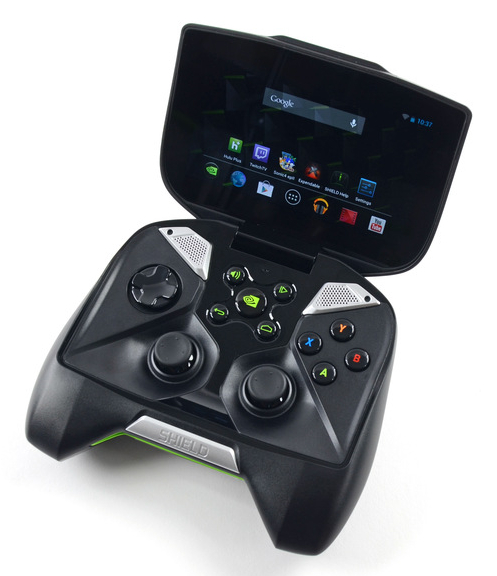
\includegraphics[width=0.3\textwidth]{Figures/nvidia-shield-open-ifixit}
  \caption[Nvidia Shield]{An open Nvidia Shield displaying the home page \cite{ImageNvidiaShield}.}
  \label{fig:nvidiashield}
\end{wrapfigure}

The Nvidia Shield game console was Nvidia's first foray into the realm of remote streaming.
Though it was focused on gaming and media streaming, it was one of the first attempts at using a portable device to stream intensive applications such as games from a host computer \cite{brown_2013}.
At the steep price point of \$349, it definitely was enthusiast hardware for a device that focused on mobile and desktop gaming over running console games or demanding titles locally.
But while the the physical device was praised for performance, battery life, and the experience of streaming games to the console, it didn't perform too well in terms of sales.
It was still widely regarded as a technological breakthrough though, and Nvidia continued to develop the technology into a new device called the Nvidia Shield TV \cite{daniel_2017}.
Focused on bringing the power of a gaming desktop to a TV, the Nvidia Shield TV dropped the idea of portability in favor of filling a different market focused on comfort.
While this is no longer a valid device for the purposes of this paper, the developments of the proprietary GameStream technology that powered the Shield and the Shield TV proved to be even more exciting than the physical devices themselves.

Though the GameStream technology that powers the Nvidia Shield devices is closed source and only officially compatible with the products Nvidia releases, its enticing power and potential drew a community to reverse engineer the protocol.
In 2013, a group of students at Case Western Reserve University developed Moonlight, an open source implementation of the GameStream protocol \cite{moonlight}.
This open source implementation allows the development of GameStream compatible clients that can run on other devices, from other computers to embedded ARM devices.
This stands as a good starting place to develop the solution described in this paper.

\section{Summary}\label{sec:StateOfTheArtSummary}

\todosection

\section{Research Questions}\label{sec:ResearchQuestions}

While there are many existing solutions for accessing a computer remotely, many struggle to be performant enough or efficient enough to stream demanding applications to the client without compromising on the user's experience.
This thesis will seek to build a solution that enables the use the power of a desktop computer from a mobile device in a way that is performant and responsive in response to the following questions:

\begin{enumerate}
  \item \textbf{Hardware Feasibility:} \emph{What hardware is needed in order to power a mobile device capable of acting as a client?}
  \item \textbf{Hardware Cost:} \emph{Is it feasible to construct such as device at a lower or comparable cost to existing solutions?}
  \item \textbf{Communication Protocol:} \emph{Does a protocol exist that is efficient enough to stream demanding applications to a client?}
  \item \textbf{Software Application:} \emph{Can a software solution be built to utilize this protocol in a manner that performant enough?}
\end{enumerate}
\chapter{Developing the Hardware} % Main chapter title

\label{Chapter4} % Change X to a consecutive number; for referencing this chapter elsewhere, use \ref{ChapterX}

\todosection

\section{Requirements}\label{sec:HardwareRequirements}

This section will explain the different constraints taken into account while developing the hardware portion of this project.
First, the hardware must be performant enough to provide a positive user experience (\ref{sec:HardwarePerformance}), and secondly the product must be cheap enough to justify it over similar alternatives (\ref{sec:HardwareCost}).

\subsection{Performance}\label{sec:HardwarePerformance}

When considering how much power needs to be incorporated in to the miniature computer, it is important to consider a number of factors, such as: having enough power to stream audio and video over the internet, not consuming too much power so as to require an expensive battery, have a fast enough connection to the internet to deliver data with the least possible latency, and having a reasonable footprint to be used as a mobile device.

Immediately, the device must be capable of decoding and rendering video that is streamed over the internet; a relatively expensive process that cannot easily be done with something such as a micro controller or even a single core CPU seen on Single Board Computers (SBC) such as the \todo{pic?}Raspberry Pi Zero.
Though at the same time, it is important to not simply build a powerful system akin to a laptop that will consume more power.
It makes no sense to built a powerful mini-computer when all it will ever be used to is to connect to another computer, and the added power draw would require a larger battery in order to stay operational for decent periods of time.
Instead it should be cut down and distilled into something that can do it's job as efficiently as possible.

The second major performance requirement of the hardware is the ability to stream this data over the internet as quickly as possible.
Because all of the data being sent to the device is live information from the host machine, the video and audio streams cannot simply be buffered in advance and played when it's ready like a recorded video.
Instead, the data must be displayed as it is received so that the user can have a smooth experience without having to wait for their keystrokes or mouse movements to be registered.
While Wi-Fi is growing ever quicker and more reliable, and should absolutely be included as a way to connected to the internet, the best way to ensure a stable and speedy connection is to use an Ethernet Cable.
This will help the device work on a consistent connection when used at a desk, while also providing a way to connect while on-the-go.

This leads to the desire for a portable design that can be used both in a conducive environnement such as a desk or while mobile.
The hardware should have the ability to be powered by a chord plugging into the device, or by an internal battery.
This alone presents a number of difficult concerns, but those will be addressed later in this chapter\todo{cite}.
Such a requirement leads to a clear benefit of integrating crucial computers such as a battery and a screen into the hardware design, while leaving as many ports open such as ethernet and USB for the user to take advantage of.


\subsection{Cost}\label{sec:HardwareCost}

Because this project consists of both a Hardware and Software component to make up a complete product, there must be reason for both to be developed.
While the software has the benefit of being the foundation for the connection between host and client machines, there are already hardware solutions that would theoretically be able to run such software.
Since the goal of this project is to save money by not needing to purchase an expensive mobile device to connect to a powerful desktop computer, there must be benefit in the hardware to warrant it's existence over repurposing something like an old laptop.
The most obvious metric of this is the actual cost of the hardware.
If the hardware can be produced at a high enough quality at a low enough cost to bring value over just a software solution, then it should be considered moving forward.
Otherwise it may prove that the development of the software should focus on compatibility so the hardware can be provided by the end user.


\section{Choosing Parts}\label{sec:ChoosingParts}

When starting to choose parts for the hardware, there are many difficult questions to face.
First and foremost, the hardware had to be built with the time and resources available for this project.
Specifically, building a Single Board Computer\todoadvisor{introduce acronyms the first time they're used}\todo{This was introduced in 4.1.1, should it also be done here?} from scratch would be completely infeasible, but the goal was also not to simply purchase an off the shelf SBC that was not tailored to the task at hand such as a traditional Raspberry Pi.
Instead, a better suited solution would be to utilize a \emph{Raspberry Pi Compute Module 4 (CM4)} which has \enquote{The power of Raspberry Pi 4 in a compact form factor for deeply embedded applications} \cite{rpi_cm4}.
Boasting an incredibly small size and streamlined I/O, there only way to communicate with the Compute Module was through two tiny mezzanine connectors as shown in Figure \ref{fig:rpi_cm4_mezzanine}.
With no other pin outs for anything such as power, HDMI, or USB, everything had to be built on a custom Printed Circuit Board (PCB).

\begin{figure}[h]
  \centering
  \begin{minipage}{0.45\textwidth}
    \centering
    \includegraphics[width=0.9\textwidth]{Figures/rpi_cm4}
    \captionsetup{width=.75\linewidth}
    \caption[Raspberry Pi Compute Module 4]{Raspberry Pi Compute Module 4, sizing\newline55 x 40mm}
    \label{fig:rpi_cm4}
  \end{minipage}\hfill
  \begin{minipage}{0.45\textwidth}
    \centering
    \includegraphics[width=0.9\textwidth]{Figures/rpi_cm4_mezzanine}
    \captionsetup{width=.75\linewidth}
    \caption[Raspberry Pi Compute Module 4 Pin out]{Close-up of the pin out, with a 0.04mm pitch between pins}
    \label{fig:rpi_cm4_mezzanine}
  \end{minipage}
\end{figure}

This PCB would have to be designed so that the CM4 could be plugged into the board using the mezzanine connectors and rely on it for all inputs and outputs.
This, however, is only the beginning of what is required to develop the product.
Since the project would not use an off the shelf SBC like a regular Raspberry PI, the project would require only designing the PCB but also picking out all the components that would go onto the PCB, such as the USB ports themselves, the USB driver chip, and related components needed for operation.
Because the CM4 is designed to be as low-powered and compact as possible, some features that would usually be expected of such a device, like the USB ports, are disabled by default and must instead be built by the board designer.
While this helps greatly by removing extraneous components and features that aren't needed for this project, it also provides me with a \todo{does this sound sarcastic?}great opportunity to learn exactly what parts are being used in the hardware.

An invaluable resource while designing the PCB was the Official I/O board for the CM4 \cite{rpi_cm4_io}.
Though the PCB board would still have to be custom built and components would need to be replaced due to the current ongoing chip shortage, it provides a great foundation instead of starting from scratch.
Another massive benefit from working within the Raspberry Pi Ecosystem is their \todo{(re)move?}incredible documentation and community surrounding the boards.
Around the time this project was being started, the CM4 was just starting to get into the hands of makers and developers, and only a couple custom boards had actually been made by anyone other than Raspberry Pi themselves.
Even though this leaves the community with less of a bulk of knowledge to work with, it has provided a sort of comradery with everyone helping each other learn the new Compute Module together.
Members of the CM4 engineering team would even assist those on the forums to help them pick parts and design their own boards.


\section{Prototyping}\label{sec:Prototyping}

Whenever working with electrical projects such as this, it is always a good idea to build up prototypes before committing to a final design that will be produced at the highest quality.
Usually breadboards and some breakout boards for Surface Mounted Devices (SMD) are a great way to develop a circuit without creating a full PCB; but due to the nature of the complex microchips required for this project as well as the dependence on the CM4's tiny mezzanine connectors, building a prototype using a breadboard is impractical given the time and resources available.
\begin{wrapfigure}{o}{0.375\textwidth}
  \centering
  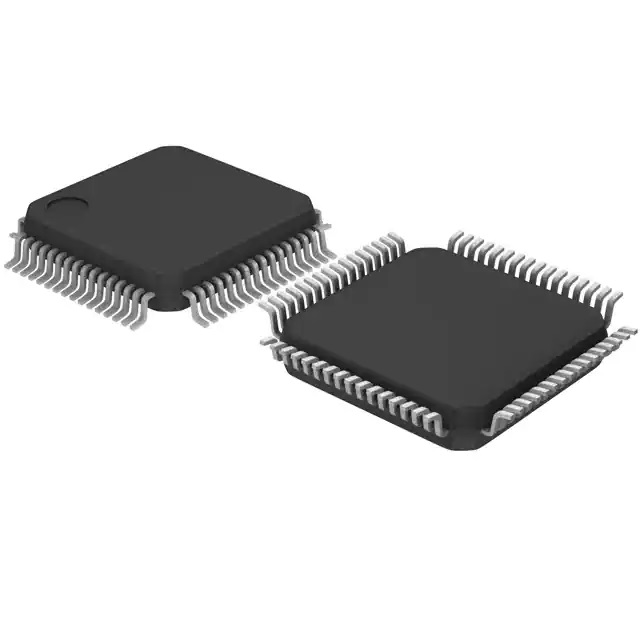
\includegraphics[width=0.3\textwidth]{Figures/64-LQFP}
  \caption[USB Controller]{The USB controller, with 0.5mm between pins}
  \label{fig:USBController}
\end{wrapfigure}
For example, the USB controller chip only has 0.5mm of space between each of it's 64 pins (Figure \ref{fig:USBController}), which would require a breakout board at least 7 times larger than the chip so that each each pin can be easily accessed by hand.
Not to mention the difficulty in wiring up that many pins along with the other related components which would need their own breakout boards either purchased or custom-designed.

\begin{figure}[h]
  \centering
  %Height instead of width because the image is rotated
  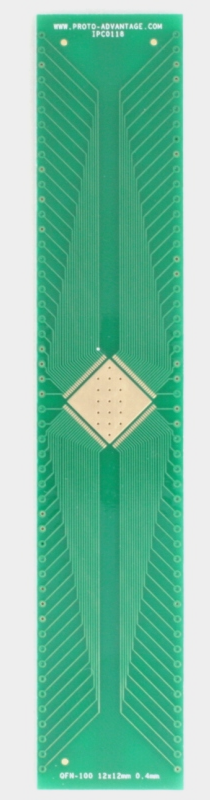
\includegraphics[height=0.9\textwidth,angle=90]{Figures/smt_breakout}
  \captionsetup{width=.8\linewidth}
  \caption[SMD Breakout Board]{A breakout board similar to what would be needer for the USB controller used on the custom PCB}
  \label{fig:smt_breakout}
\end{figure}

Instead, the first board was built out in a piecewise fashion, allowing each section of the board a way to fail without interrupting the rest of the board.
This allows each function of the board to be tested individually and in isolation so that changes could be made incrementally without needing to worry about their integration with the rest of the board.
\todo{convert first person to third person}For example, in order to build a system that would allow the board to be powered via USB or an internal battery, as well as charge the battery simultaneously, I would need to build a complex circuit consisting of parts neither I nor anyone I knew had used before.
Since power is obviously a critical component of the board, A secondary way of feeding power directly the board was built to bypass all that circuitry in case it fails.
In doing so, the board can still be powered and it's other features can be tested while a fix for that portion of the circuitry is developed for the next iteration.


\section{Designing the Printed Circuit Board}\label{sec:DesigningThePCB}

\todosection


\section{Manufacturing the Circuit Board}\label{sec:ManufacturingThePCB}

\todosection
\chapter{Developing the Software} % Main chapter title

\label{Chapter5} % Change X to a consecutive number; for referencing this chapter elsewhere, use \ref{ChapterX}

\todosection


\section{Requirements}\label{sec:SoftwareRequirements}

Much like the hardware requirements in section \ref{sec:HardwareRequirements}, the primary requirement of the software is to be performant enough to provide the user with a positive experience.
This is broken down to include being able to stream and decode video over the internet with as little latency as possible, stream inputs from the user to the remote computer, and retain visual fidelity while the host machine is under heavy load.
While much of the latency between the host and client is due to the network both devices are connected to, there is still some optimizations that can be made to reduce the time between data being send and images being displayed on the screen.
Similarly, while the rate at which data is transferred between the host and client cannot exceed the speed of the slowest internet connection of the two devices, there can still be a balance between the bandwidth-saving but lower quality streaming seen in Chrome Remote Desktop (\ref{subsec:ChromeRemoteDesktop}), and the local network but higher quality Nvidia Shield (\ref{subsec:NvidiaShieldAndGameStream}).
To accomplish this, a compression method similar to CRD will be used, but it will not be bound by the traditional web browser which limit CRD due to the software solution being developed as a native application.

As a secondary objective, it would also be beneficial for the software to be able to run on a variety of different hardware platforms in the event the hardware is determined to be infeasible to develop, as discussed in Section \ref{subsec:HardwareCost}.


\section{Potential Avenues}\label{sec:PotentialAvenues}

As with any software project, there are many potential ways to solve the problem.
In many cases, the easiest place to start is to begin by ruling out potential avenues that are not feasible.
For example, as evident by the number of existing solutions that attempt to solve this problem (Chapter \ref{Chapter3}), taking into special account Nvidia's recent foray into remote gaming with the Shield (\ref{subsec:NvidiaShieldAndGameStream}), it is not reasonable to attempt to create a brand new software solution from scratch with the time and resources available.
It has taken Nvidia, a company worth hundreds of billions of dollars, years to get to the point they are at now \cite{brown_2013}.
Developing a rival protocol or new software platform is simply not possible for this project.
Instead, given that Nvidia's GameStream technology is the current leader in the realm of high-performance remote computing, the best way to build a software product that meets the requirements laid out in Section \ref{sec:ResearchQuestions} is to build upon what already exists.


\subsection{NVIDIA GameStream}\label{subsec:NVIDIAGameStream}

\todo[linecolor=green,backgroundcolor=green!25,bordercolor=green,inline]{Should this subsection and the following subsection be top level sections? The organization of the headers is a little strange, but the content flows pretty well}

Unfortunately, the Nvidia GameStream protocol is both proprietary and a closed source project.
Very little is officially known about the protocol, other than it uses specific video encoders built into Nvidia Graphics cards from the 600 series from 2012 and newer \cite{gamestream_userguide}.
Apart from that, everything has been researched and reverse engineered by the community.
A GameStream session is started by first connecting to a host computer which has enabled the GameStream service through Nvidia's GeForce Experience application.
Once the service is enabled, the computer will listen on port \emph{47989}\todoquestion{Should this be italicized? quoted? plaintext?} for the following web requests:
\begin{itemize}
  \item /serverinfo
  \item /pair
  \item /unpair
  \item /applist
  \item /launch
  \item /resume
  \item /cancel
\end{itemize}
Once a session has been started with a \emph{/launch} request, raw data covering video, audio, and input is passed back and forth over a number of ports until the session is terminated.
An end-to-end example of the protocol's usage is as follows:

\begin{enumerate}
  \item A user knows that a capable host computer is ready to stream at the address \emph{192.168.1.123}.
        \begin{enumerate}
          \item This can be confirmed by sending a HTTP GET request \emph{/serverinfo} to the host computer on port \emph{47989}. For example: \newline\emph{http://192.168.1.123:47989/serverinfo?uniqueid=1234}
        \end{enumerate}
  \item The user can make a request to \emph{/pair} with a number of parameters to authorize itself with the host.
        \begin{enumerate}
          \item Pairing is a two step-process.
                First, a request to pair is made, at which point the host machine will display a four digit code on it's screen.
                Then the client must send that code back to the host as a second form of authentication.
          \item The authentication created by this pairing process lasts until either the client makes an \emph{/unpair} request with it's unique ID or a user on the host machine unpairs the client.
        \end{enumerate}
  \item The user can make a request to \emph{/applist} to get a list of applications that the host is able to stream.
  \item The user makes a request to \emph{/launch} with a number of parameters to instruct the host to create a session with the given settings and launch the specified application.
        \begin{enumerate}
          \item The configuration options given include the application to launch, the video resolution to stream, audio setup, input mapping, and multiple forms of authentication.
        \end{enumerate}
  \item If the user unexpectedly or accidentally leaves a session without closing it, they can make a request to \emph{/resume} to instruct the host to reopen and resume the session the previous session.
  \item Once the user is finished, they make a request to \emph{/cancel} to instruct the host to close the session.
  \item If the user is completely finished with the host, they can return it to the state they found it in by making a request to \emph{/unpair} with their unique ID, unauthorizing themselves with the host.
\end{enumerate}

The most difficult part of this process is handling the transfer of data after a session has begun.
Once a session has launched, data is sent directly between the host and client over a number of ports without going through an easy to understand web protocol.
This is where the community project Moonlight steps in.

\subsection{Moonlight}\label{subsec:Moonlight}

Moonlight is an unofficial third-party open-source client for the Nvidia GameStream protocol \cite{moonlight}.
The project is structured as a core library written in \emph{C} with a number of community built clients built on top of it for various platforms.
In essence, it turns the process described in the previous section (\ref{subsec:NVIDIAGameStream}) into a usable API.
By reverse engineering the protocol originally implemented by the Nvidia Shield, Moonlight enables the development of a GameStream client for any other platform.
The Moonlight community has already developed fantastic clients for many platforms such as Windows, Mac, Linux, Android, iOS, Web, and even other gaming consoles.
All that is needed for the purposes of this project is to make tweaks to best suit the CM4 that drives the hardware and develop a suite of tools to test it's functionality.


\section{Developing for ARM}\label{sec:DevelopingForARM}

\todosection


\section{Developing Testing and Measurement Tools}\label{sec:DevelopingTestingAndMeasurementTools}

\todosection
\chapter{Evaluation} % Main chapter title

\label{Chapter6} % Change X to a consecutive number; for referencing this chapter elsewhere, use \ref{ChapterX}


\section{Testing Methodology}

\todosection


\section{Responsivity and Latency}

\todosection


\section{Performance}

\todosection


\section{Quality}

\todosection


\section{Summary}

\todosection
\chapter{Conclusion}

\label{Chapter7}


\section{Summary}\label{sec:ConclusionSummary}

This thesis has proved that it is possible to produce a hardware and software solution that is capable of leveraging the power of a desktop computer remotely without sacrificing the user's experience.
It improves upon existing solutions by continuing to offer a performant and high-quality stream of the host's screen and audio to the user even as the host is running highly demanding applications.
Each of the questions posed in Section \ref{sec:ResearchQuestions} can be answered individually.

\begin{enumerate}
  \setcounter{enumi}{0} % Start the enumeration at X+1
  \item \textbf{Hardware Feasibility:} \emph{What hardware is needed in order to power a mobile device capable of acting as a client?}
\end{enumerate}

\noindent
This thesis project is able to run on embedded Single Board Computers and hardware available for purchase today.
While this project built a custom PCB for the Raspberry Pi Compute Module 4 (Discussed in section \ref{sec:ChoosingParts}), the software could also run on consumer-grade Raspberry Pi models as well.

\begin{enumerate}
  \setcounter{enumi}{1} % Start the enumeration at X+1
  \item \textbf{Hardware Cost:} \emph{Is it feasible to construct such as device at a lower or comparable cost to existing solutions?}
\end{enumerate}

\noindent
Yes, the total cost for a single hardware unit, including the board and all its components, totalled in under \$150, and could even be produced for less (Discussed in Section \ref{subsec:HardwareCost}).
This cost is considerably cheaper than buying a new laptop device, and often cheaper than buying a used laptop with comparable power.

\begin{enumerate}
  \setcounter{enumi}{2} % Start the enumeration at X+1
  \item \textbf{Communication Protocol:} \emph{Does a protocol exist that is efficient enough to stream demanding applications to a client?}
\end{enumerate}

\noindent
Yes, Nvidia's GameStream protocol proved itself to be capable of streaming highly demanding applications to a client device without any loss of quality or performance (Discussed in Section \ref{sec:EvaluationSummary}).
Even though it's original purpose and namesake is to stream video games, the high demands of such a use case have made it applicable to much more than just that.
While Microsoft's Remote Desktop Protocol proved to be powerful enough to stream demanding applications to a client device, it's limitations and closed-source nature prevent it from being the viable solution for certain use cases (Discussed in \ref{subsec:RemoteDesktopProtocol}).

\begin{enumerate}
  \setcounter{enumi}{3} % Start the enumeration at X+1
  \item \textbf{Software Application:} \emph{Can a software solution be built to utilize this protocol in a manner that performant enough?}
\end{enumerate}

\noindent
Yes, the solution produced in this thesis is built upon the open source project Moonlight, which utilizes the GameStream protocol, to provide a software application that is capable of streaming demanding applications to a client device while remaining performant enough to provide a positive user experience (Discussed in Section \ref{sec:EvaluationSummary}).


\section{Limitations}\label{sec:ConclusionLimitations}

While this thesis was constructed with the utmost attentiveness with regards to the time and resources available, there are still limitations in what could be accomplished.
The largest limitation is the lack of testing in alternative environments.
All of the testing performed in Chapter \ref{Chapter6} was performed in an ideal network environment, where there was minimal network latency between the host and client machines due to them both being connected to the same network by ethernet.
While this is a good indicator of the best possible performance, it is not very indicative of the performance that could be expected in a real-world environment.
More testing should be done where the host and client machines are located on different networks akin to the use case described in Section \ref{sec:ApplicationToModernDay}.

Secondly, due to the ongoing chip shortage and the lack of experience in developing PCB boards, it is very likely that there are better ways to develop the PCB board for this project.
While the board was able to meet the requirements for this project, there we're many instances (some described in table \ref{tab:SelectedComponents}) where alternative parts had to be chosen and designed around because the first-choice was out of stock.
It is very possible that the board could have been constructed quicker and at a cheaper price if more parts were available for purchase.


\section{Future Research}\label{sec:ConclusionFutureResearch}

Should this project be continued in the future, there are multiple ways that additional time and resources could further improve this project.
The first improvement to make is to fix the issue with USB data described in section \ref{subsec:Manufacturing3}.
This is the only flaw in the hardware preventing it from being considered a completed product.
Similar to the previous section, if more time were available, more testing could be done in various environments to identify any weaknesses in the software that may have gone unnoticed.

Another aspect of the project worth testing in more detail is the performance of the hardware produced in Chapter \ref{Chapter4} compared to the hardware performance of the development board that is sold with the CM4 (Section \ref{sec:ChoosingParts}).
The ideal outcome is that the two boards provide the same performance, meaning that there is no unneeded overhead introduced by the board produced in this thesis that should be fixed.
In the event that there is slowdown somewhere within the custom board, the specific problem should be identified and redesigned to provide optimal performance.

After experimenting with streaming over different networks and testing the project under different conditions, it would be beneficial to look at polishing the hardware of the project into a self-contained product.
As it stands, it is currently a PCB with peripherals attached that make it cumbersome to carry around.
The groundwork for this has already been laid out in Section \ref{subsec:DesigningHDMI}, with FFC connectors established for one HDMI and one USB port for connection to an embedded screen, and with the footprint of the final PCB and battery fitting within the footprint of the chosen screen.
All that is left is to build an enclosure to house the final product.

%----------------------------------------------------------------------------------------
%	THESIS CONTENT - APPENDICES
%----------------------------------------------------------------------------------------

\appendix % Cue to tell LaTeX that the following "chapters" are Appendices

% Include the appendices of the thesis as separate files from the Appendices folder
% Uncomment the lines as you write the Appendices

\chapter{PCB Specifications} % Main appendix title

\label{AppendixA} % For referencing this appendix elsewhere, use \ref{AppendixA}

\section{PCB Schematic}

\begin{figure}[h]
  \centering
  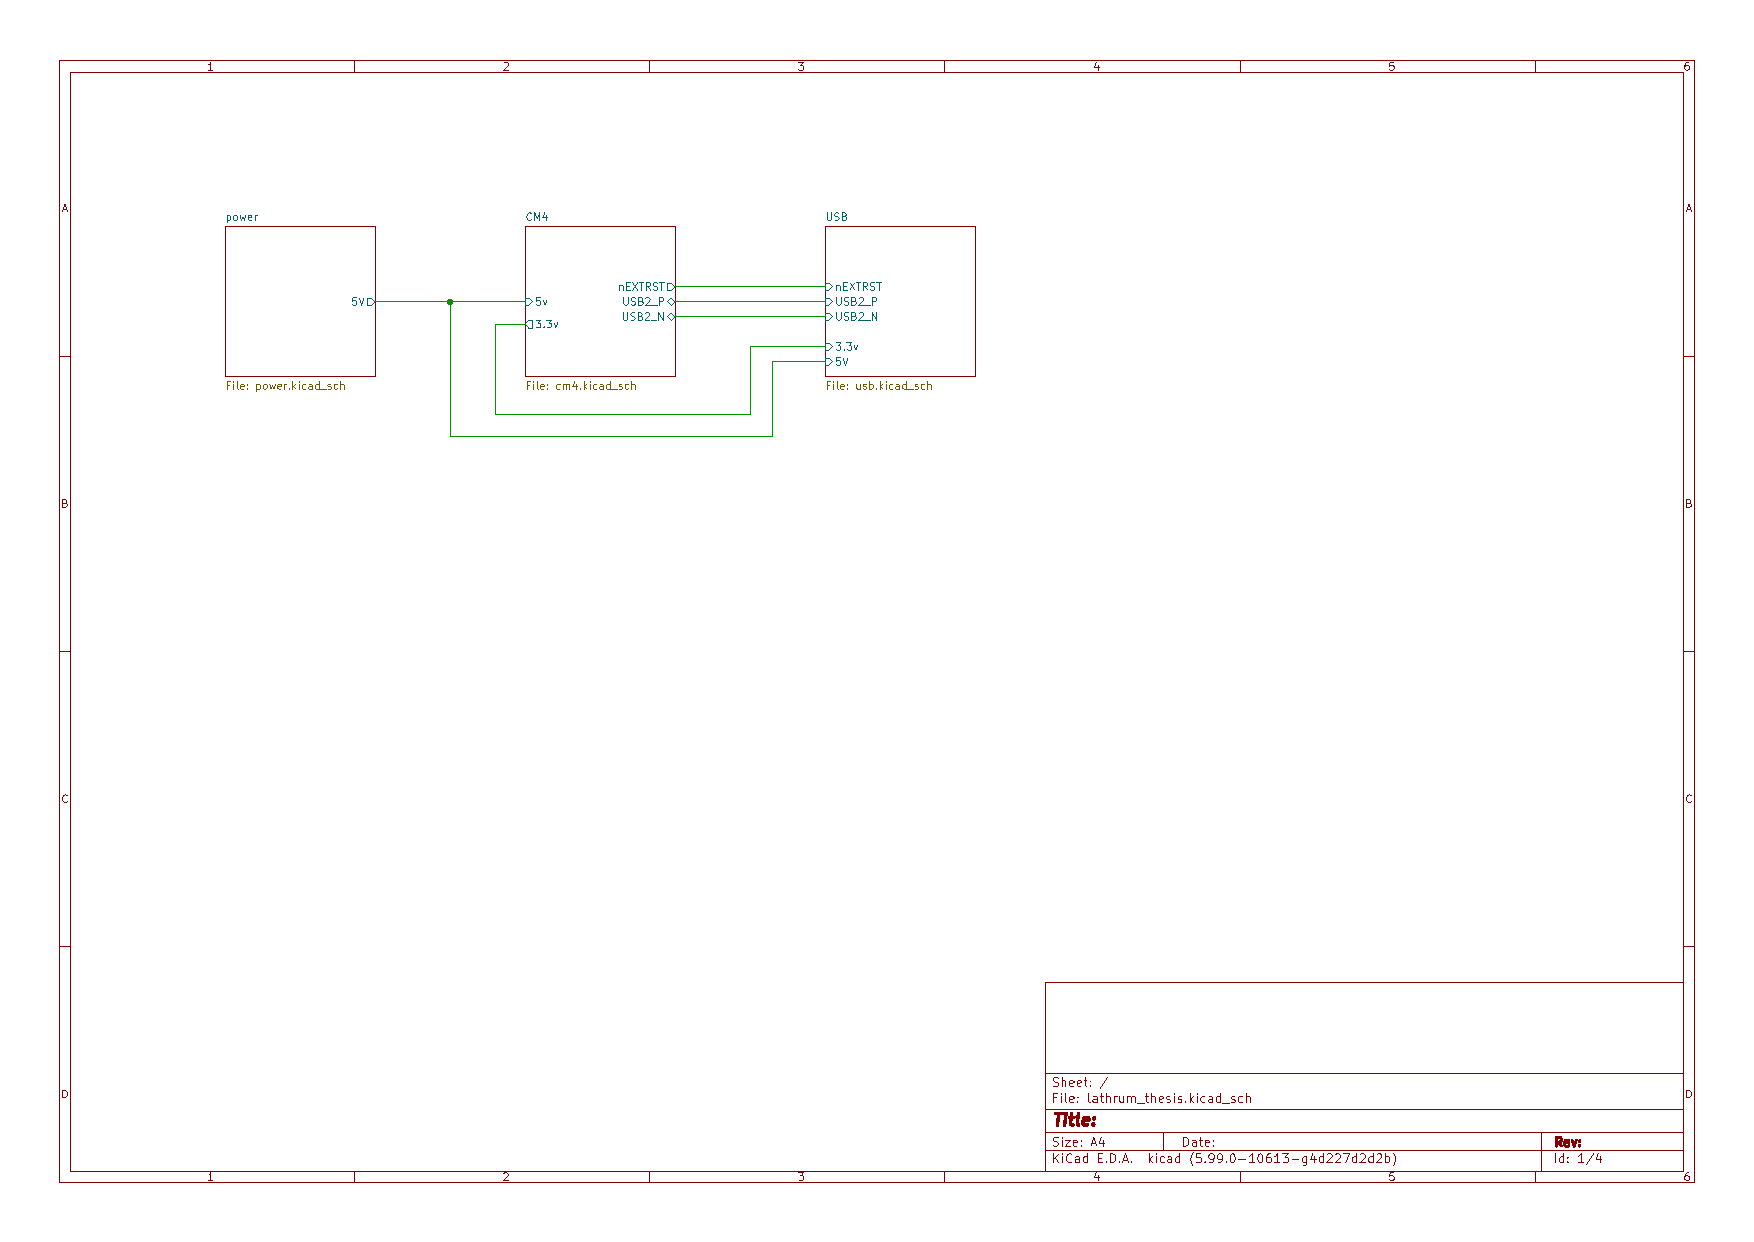
\includegraphics[width=1\textwidth,page=1]{Figures/kicad/lathrum_thesis_schematic.pdf}
  \captionsetup{width=.8\linewidth}
  \caption[Top Level Schematic]{The top level of the PCB board schematic}
  \label{fig:pcb_schematic_top}
\end{figure}

\begin{figure}[h]
  \centering
  \includegraphics[width=1\textwidth,page=2]{Figures/kicad/lathrum_thesis_schematic.pdf}
  \captionsetup{width=.8\linewidth}
  \caption[Power Schematic]{Schematic layout for the power circuit, including battery management}
  \label{fig:pcb_schematic_battery}
\end{figure}

\begin{figure}[h]
  \centering
  \includegraphics[width=1\textwidth,page=3]{Figures/kicad/lathrum_thesis_schematic.pdf}
  \captionsetup{width=.8\linewidth}
  \caption[CM4 Schematic]{Schematic layout for interfacing with the Compute Module 4}
  \label{fig:pcb_schematic_cm4}
\end{figure}

\begin{figure}[h]
  \centering
  \includegraphics[width=1\textwidth,page=4]{Figures/kicad/lathrum_thesis_schematic.pdf}
  \captionsetup{width=.8\linewidth}
  \caption[USB Schematic]{Schematic layout for the USB hub and ports}
  \label{fig:pcb_schematic_usb}
\end{figure}

% Make sure next section is on a new page
\clearpage
\section{PCB Layout}

\begin{figure}[h]
  \centering
  %Height instead of width because the image is rotated
  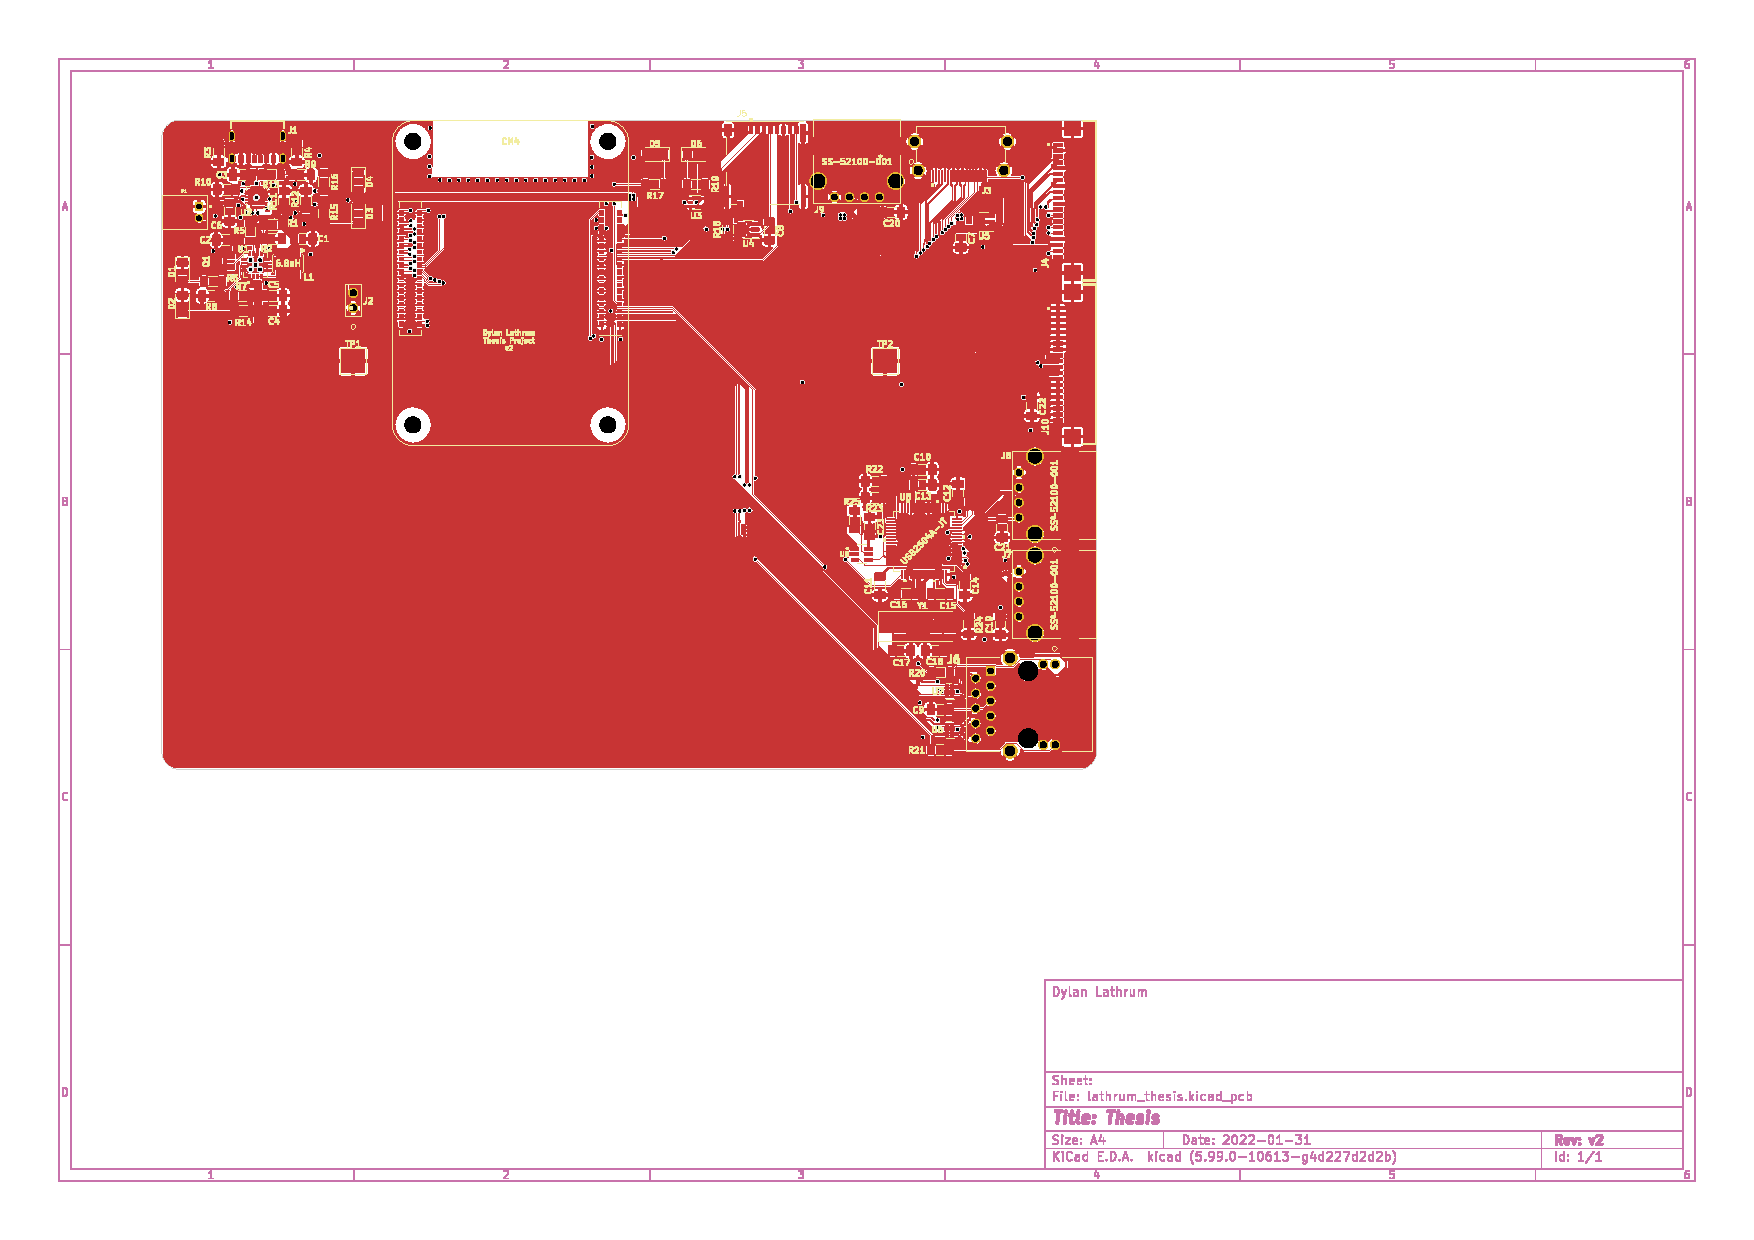
\includegraphics[height=0.9\textwidth,angle=90,page=1]{Figures/kicad/lathrum_thesis_layout_front.pdf}
  \captionsetup{width=.8\linewidth}
  \caption[PCB Front Layout]{Physical board layout for the front side of the PCB}
  \label{fig:pcb_layout_front}
\end{figure}

\begin{figure}[h]
  \centering
  %Height instead of width because the image is rotated
  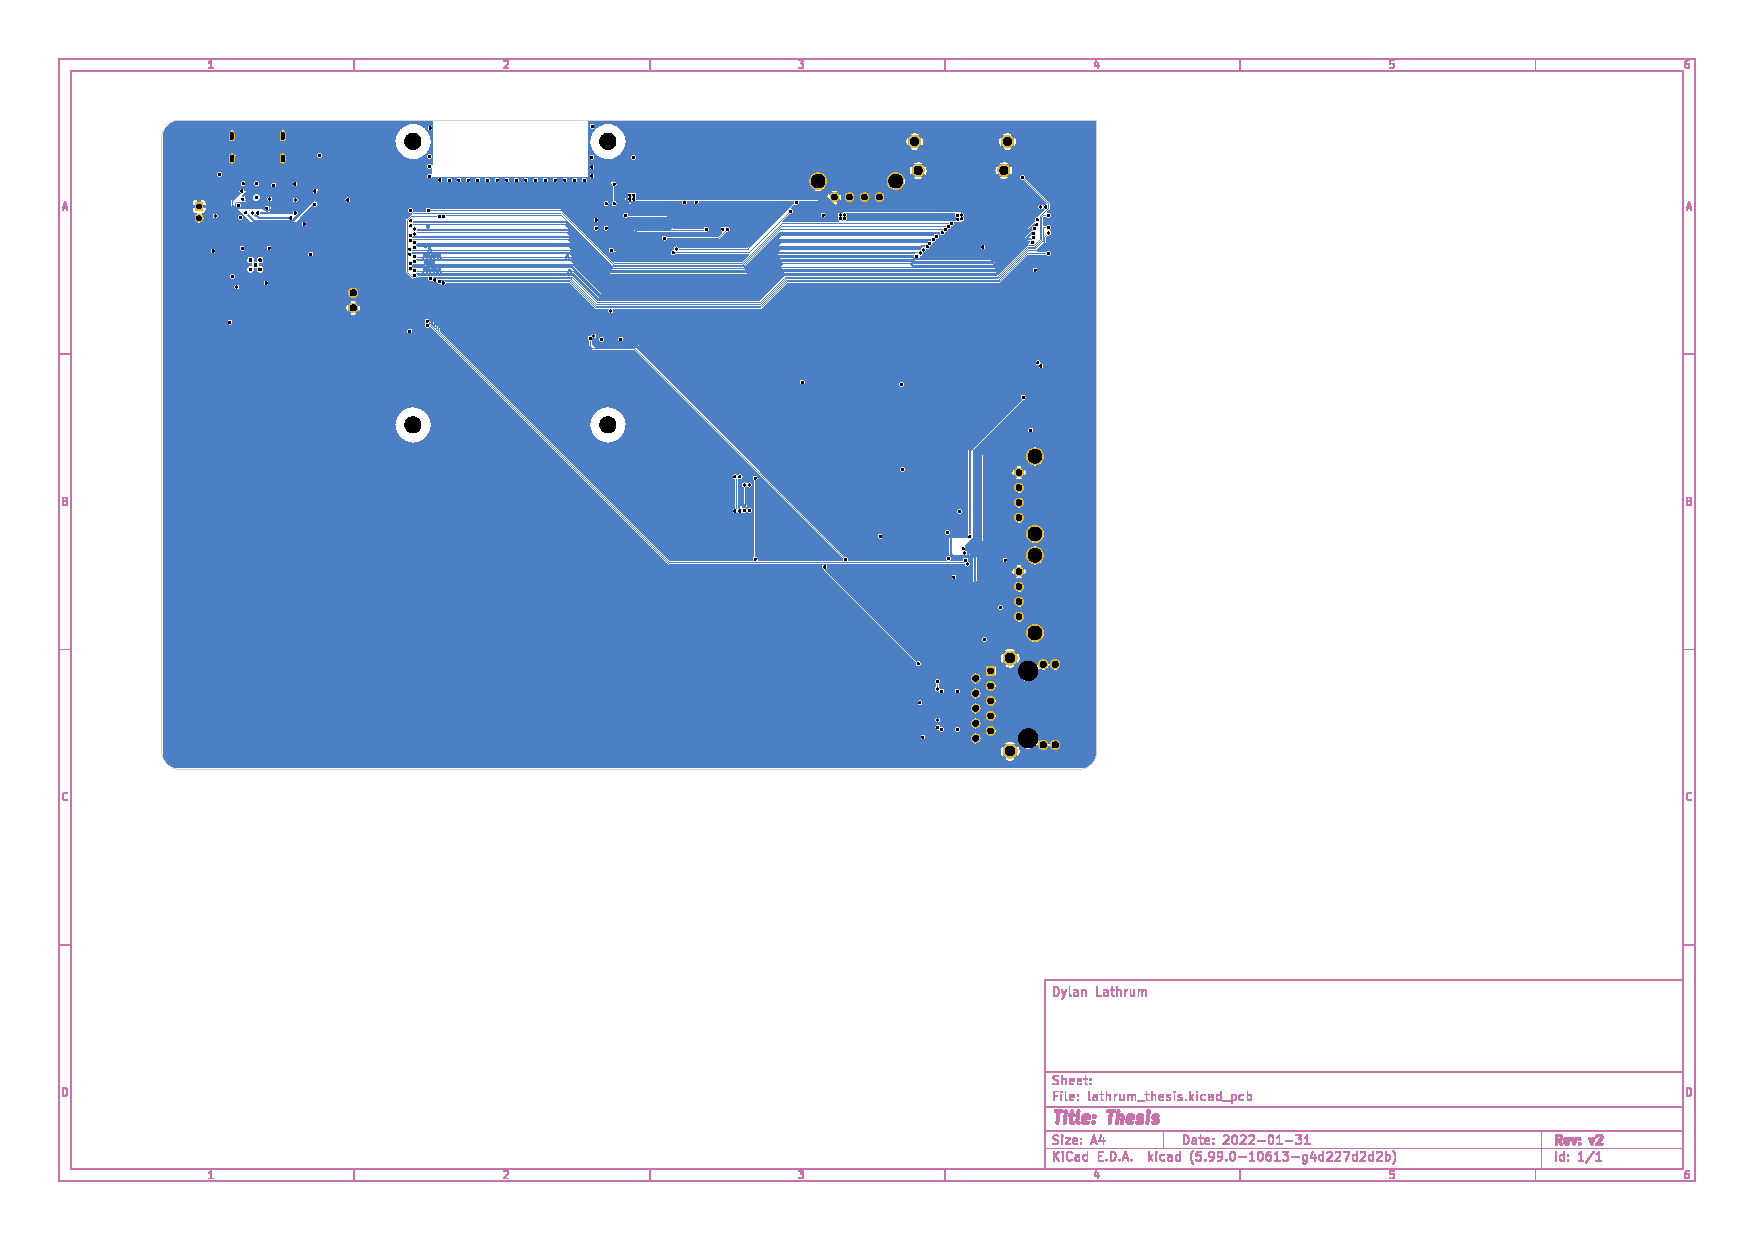
\includegraphics[height=0.9\textwidth,angle=90,page=1]{Figures/kicad/lathrum_thesis_layout_back.pdf}
  \captionsetup{width=.8\linewidth}
  \caption[PCB Back Layout]{Physical board layout for the back side of the PCB}
  \label{fig:pcb_layout_back}
\end{figure}
\chapter{Bill of Materials} % Main appendix title

\label{AppendixB} % For referencing this appendix elsewhere, use \ref{AppendixA}

\begin{longtable}{|>{\raggedright\arraybackslash}p{0.2\linewidth}|c|l|l|}%
  \hline
  \bfseries Reference \newline Designator& \bfseries Count & \bfseries Manufacturer's Number &\bfseries Value % Columns
  \csvreader[respect percent=true, respect underscore=true, respect sharp=true, table head=\toprule, table foot=\bottomrule]{Figures/kicad/lathrum_thesis_bom.csv}{}% Data
  {\\\hline\csvcoli&\csvcolii&\csvcolv&\csvcoliii}% Rows
  \\\hline
  \caption[Bill of Materials]{Bill of Materials for a single PCB Board.}
  \label{tab:BillOfMaterials}
\end{longtable}
\chapter{Open Source Repository} % Main appendix title

\label{AppendixC} % For referencing this appendix elsewhere, use \ref{AppendixA}

The entirety of this project, including hardware schematics and software code, is available online on GitHub at: \url{https://github.com/Dylancyclone/thesis}.

%----------------------------------------------------------------------------------------
%	BIBLIOGRAPHY
%----------------------------------------------------------------------------------------

\printbibliography[heading=bibintoc]

%----------------------------------------------------------------------------------------

\end{document}
